\apendice{Especificación de diseño}

\section{Introducción}
En este apartado del anexo se van a documentar todos los aspectos relacionados al diseño del proyecto, y como consecuencia, de la aplicación desarrollada en el mismo. Se describirán los componentes y entidades que forman el proyecto, y cómo estos se relacionan entre sí, con el objetivo de detallar cómo logran implementar los objetivos del proyecto ya mencionados.

La manera principal de explicar los componentes, datos y entidades del diseño del proyecto será la de varios diagramas que ayuden a comprender el funcionamiento y relaciones que existen entre los mismos, incluyendo sus atributos y características.

\section{Diseño de datos}

En esta sección se describirá el diseño de los datos del sistema. Para ello se detallará una serie de diagramas entidad-relación que detallarán cómo se relacionan estos entre sí, mostrando los atributos más influyentes de cada uno. 

\begin{figure}[H]
\centering
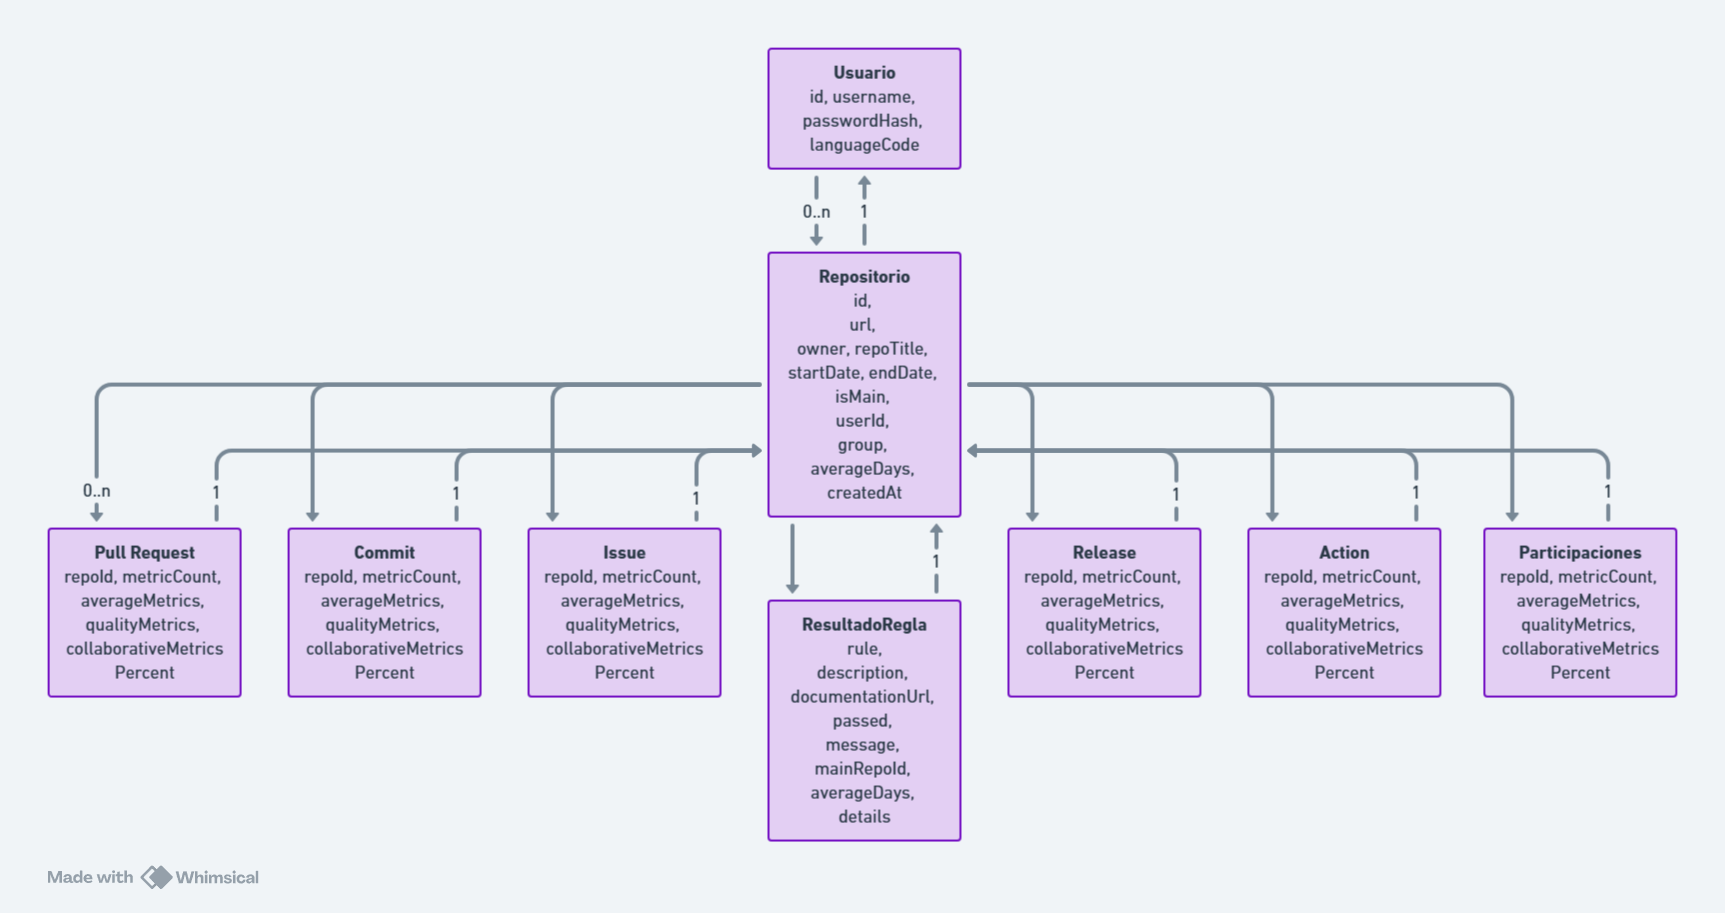
\includegraphics[width=0.8\textwidth]{img/Diagrama-entidad-relacion.png}
\caption{Diagrama Entidad - Relación de la aplicación del proyecto}
\label{fig:DiagramaER}
\end{figure}

\begin{figure}[H]
\centering
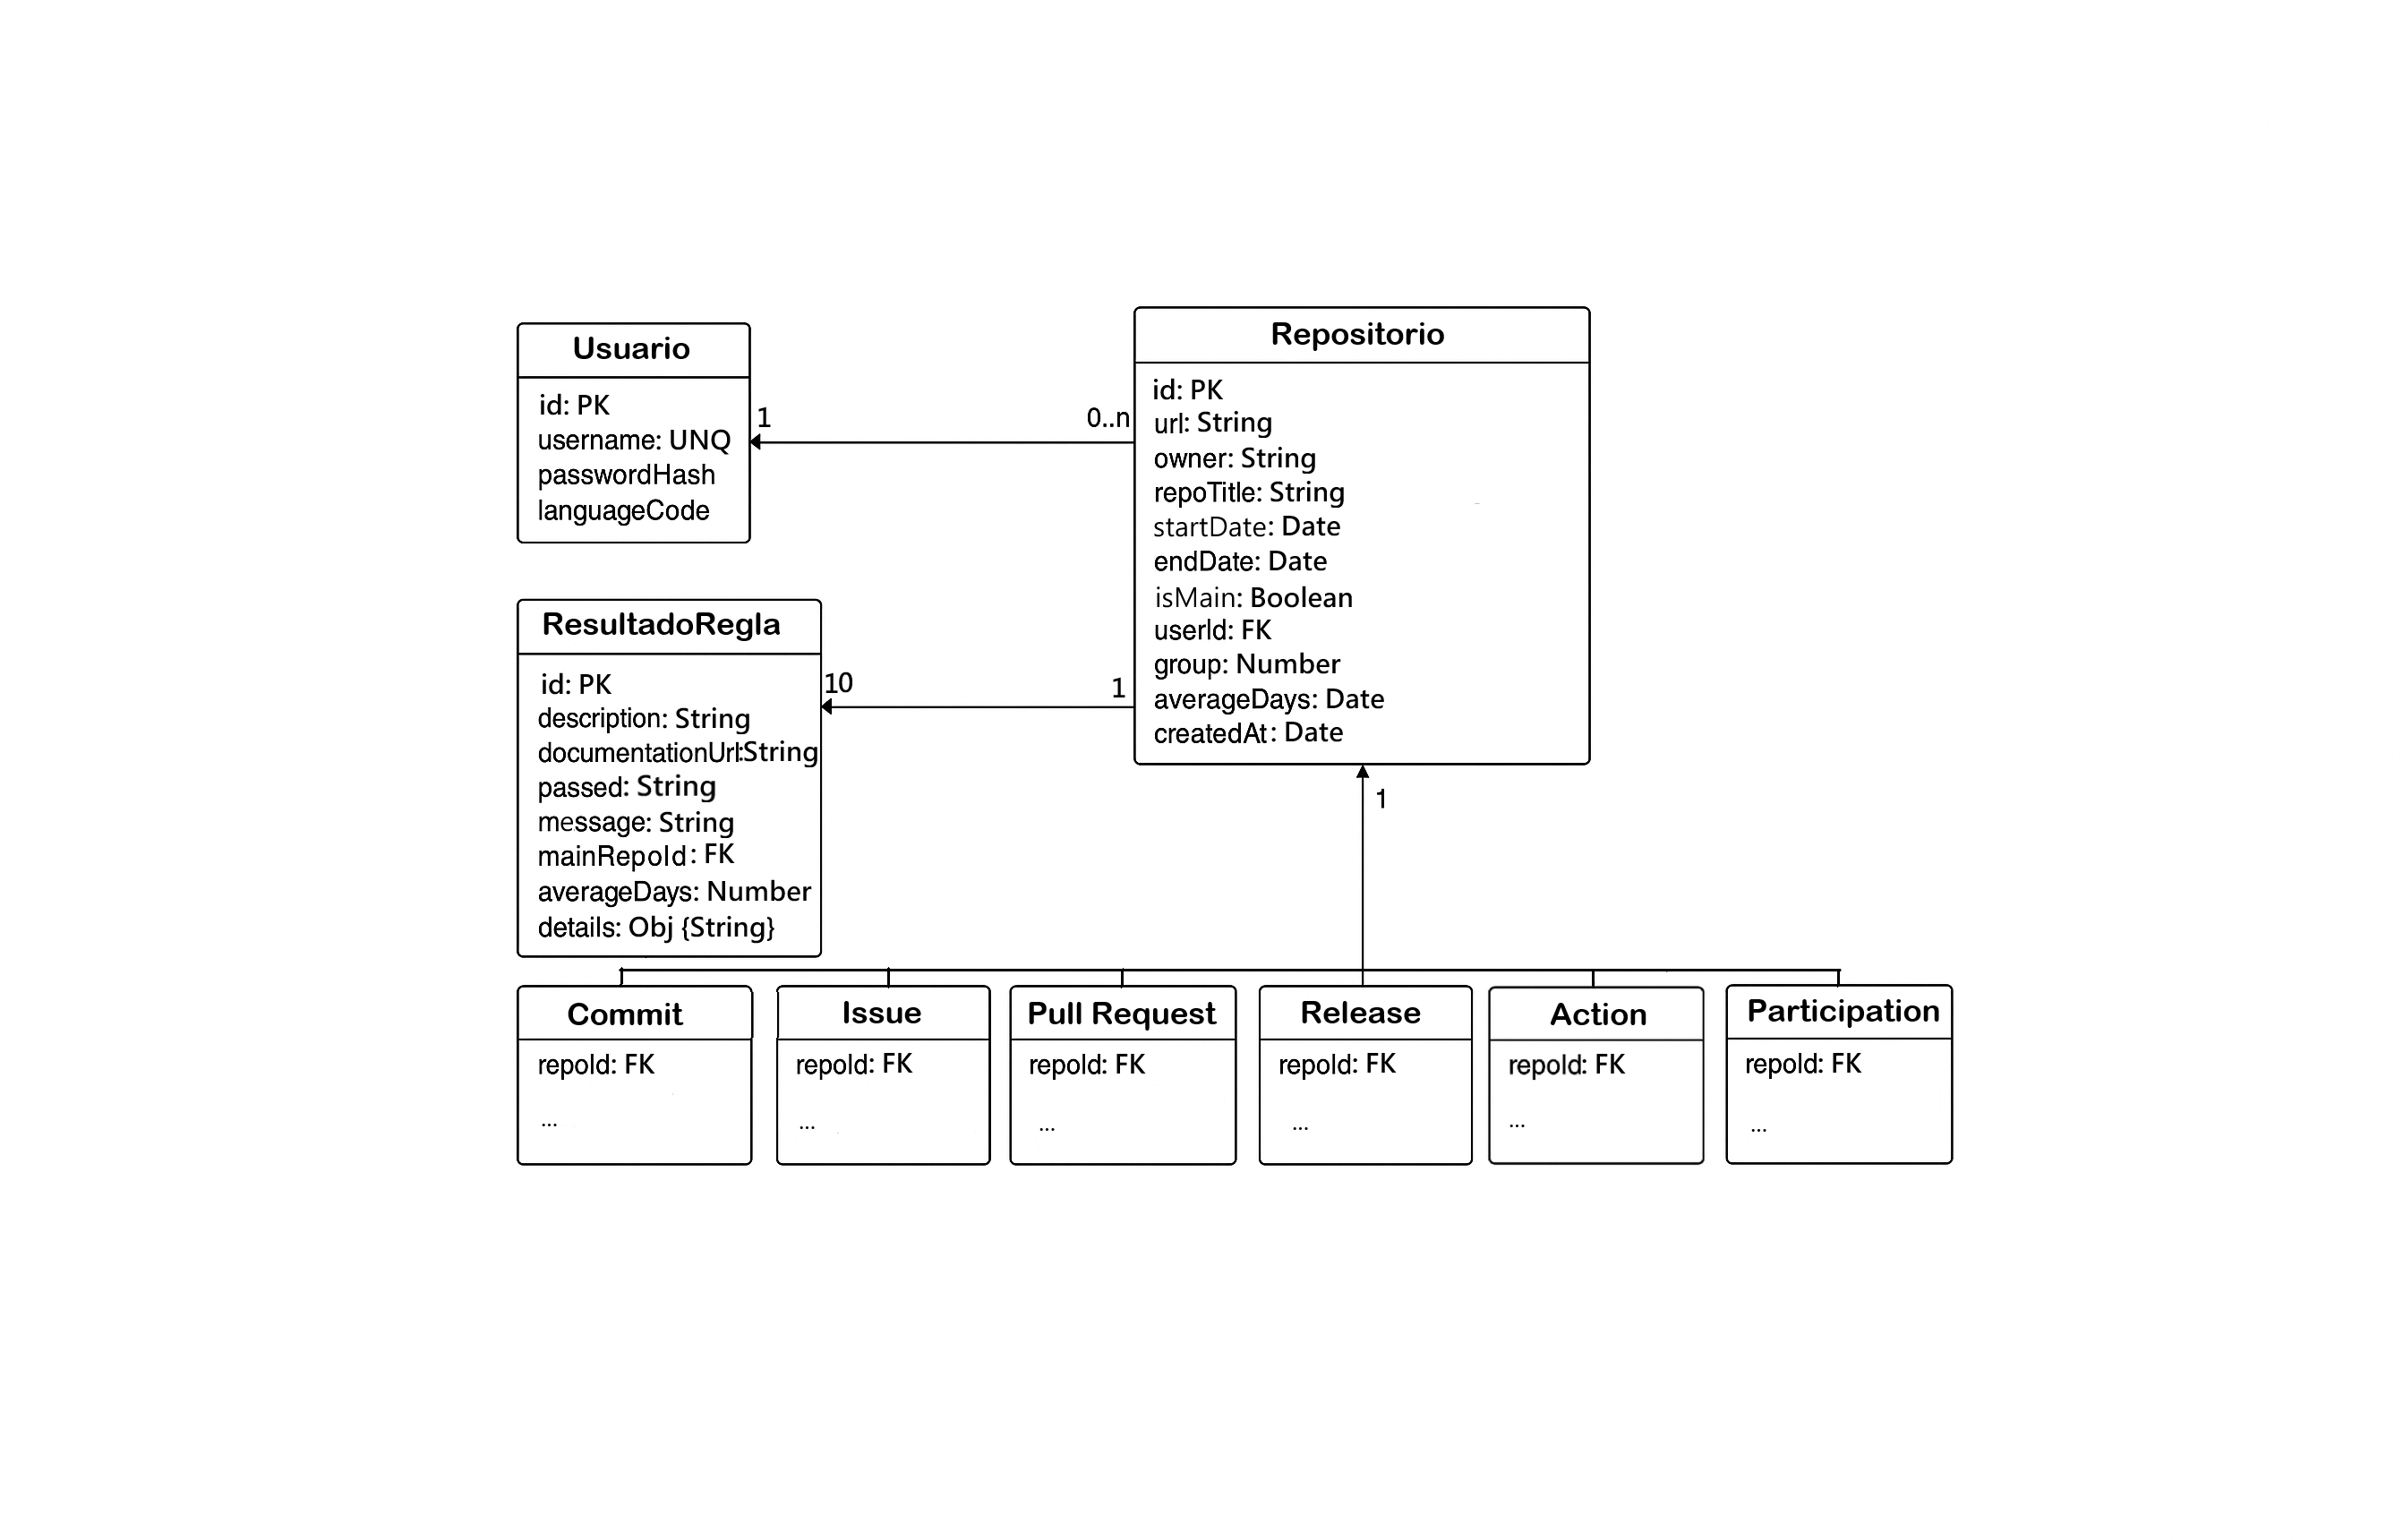
\includegraphics[width=0.8\textwidth]{img/Diagrama-entidad-relacionUML.png}
\caption{Diagrama Entidad - Relación UML de la aplicación del proyecto}
\label{fig:DiagramaER_UML}
\end{figure}

\subsection{Entidades del Sistema}
\begin{itemize}
	\item \textbf{Usuario}: Representa a los usuarios de la aplicación.
		\begin{itemize}
			\item \textbf{id}: Identificador único del usuario.
			\item \textbf{username}: Nombre de usuario, único en el sistema.
			\item \textbf{passwordHash}: Contraseña encriptada.
			\item \textbf{languageCode}: Código del idioma que utiliza el usuario.
		\end{itemize}

	\item \textbf{Repositorio}: Contiene los datos de un repositorio analizado.
		\begin{itemize}
			\item \textbf{id}: Identificador único del repositorio analizado.
			\item \textbf{url}: Dirección URL del repositorio.
			\item \textbf{owner}: Nombre del propietario del repositorio.
			\item \textbf{repoTitle}: Título o nombre del repositorio.
			\item \textbf{startDate}: Fecha de inicio del análisis.
			\item \textbf{endDate}: Fecha de finalización del análisis.
			\item \textbf{isMain}: Indica si es el repositorio principal o de referencia.
			\item \textbf{userId}: Identificador del usuario propietario del repositorio.
			\item \textbf{group}: Número de grupo comparativo de referencia (si aplica).
			\item \textbf{averageDays}: Número de días promedio utilizado en métricas de media.
			\item \textbf{createdAt}: Fecha de creación del análisis.
		\end{itemize}

	\item \textbf{ResultadoRegla}: Almacena el resultado del análisis de buenas prácticas.
		\begin{itemize}
			\item \textbf{rule}: Nombre de la regla evaluada.
			\item \textbf{description}: Descripción de la regla.
			\item \textbf{documentationUrl}: Enlace a la documentación de la regla.
			\item \textbf{passed}: Indica si la regla fue superada.
			\item \textbf{message}: Comentario asociado al resultado.
			\item \textbf{mainRepoId}: Repositorio principal evaluado.
			\item \textbf{averageDays}: Días promedio utilizados en la evaluación.
            \item \textbf{details}: Medidas que evalúa la regla y su evaluación
		\end{itemize}

	\item \textbf{Métricas (\textit{Commit}, \textit{Issue}, \textit{Pull Request}, \textit{Release}, \textit{Action}, \textit{Participaciones}}: Cada una de estas entidades representa métricas agregadas de su tipo específico, siempre vinculadas a un único repositorio mediante la clave \textbf{repoId}.
		\begin{itemize}
			\item \textbf{repoId}: Repositorio al que pertenece la métrica.
			\item \textbf{metricCount}: Total numérico de la métrica (Por ejemplo \textit{commitCount}).
			\item \textbf{averageMetrics}: Promedio de aparición o cierre de la métrica (Por ejemplo averageClosedIssues).
			\item \textbf{qualityMetrics}: Atributos que reflejan medidas de calidad de proceso que dependen del tipo de métrica (Por ejemplo el porcentaje de issues con imágenes, o el número de ficheros workflow ejecutados con éxito).
			\item \textbf{collaborativeMetricsPercent}: Porcentaje de instancias de la métrica realizadas de forma colaborativa.
		\end{itemize}
    \end{itemize}

\subsection{Relaciones entre Entidades}
\begin{itemize}
	\item \textbf{Usuario - Repositorio}:
	\begin{itemize}
		\item Un \textbf{Usuario} posee \textbf{0..n} instancias de \textbf{Repositorio}.
		\item Un \textbf{Repositorio} pertenece a exactamente un \textbf{Usuario}.
	\end{itemize}

    \item \textbf{Repositorio - ResultadoRegla}:
	\begin{itemize}
		\item Un \textbf{Repositorio (principal)} genera \textbf{10} resultados de \textbf{ResultadoRegla} (Uno por cada una de las 10 reglas definidas).
		\item Un \textbf{ResultadoRegla} se asocia a exactamente un \textbf{Repositorio (principal)}.
	\end{itemize}

	\item \textbf{Repositorio - Métrica}:
	\begin{itemize}
		\item Un \textbf{Repositorio} tiene exactamente una instancia de métricas para cada uno de los siguientes: \textbf{\textit{Commit}}, \textbf{\textit{Issue}}, \textbf{\textit{Pull Request}}, \textbf{\textit{Release}}, \textbf{\textit{Action}}, \textbf{Participaciones}.
		\item Cada una de estas métricas pertenece a un solo \textbf{Repositorio}.
	\end{itemize}
\end{itemize}

\section{Diseño arquitectónico}

El diseño de la arquitectura de la aplicación se divide en 2 partes fundamentales: un frontend de Angular dividido en componentes y servicios, y un backend de Node js que usa controladores para ejecutar funciones y modelos para la base de datos. La separación del frontEnd y el backend garantiza la separación de responsabilidades, lo que se ve reforzado por los componentes del frontend y los controladores del backend, que separan aún más las reponsabilidades internamente. Los componentes y controladores siguen el principio \textit{Open-Closed} de programación, permitiendo añadir nuevas funcionalidades sin necesidad de alterar el resto del código (Por ejemplo añadir nuevas pantallas o reglas).

Esta arquitectura y sus divisones en directorios se muestran de una forma más detallada y visual en la siguiente figura:

\begin{figure}[H]
\centering
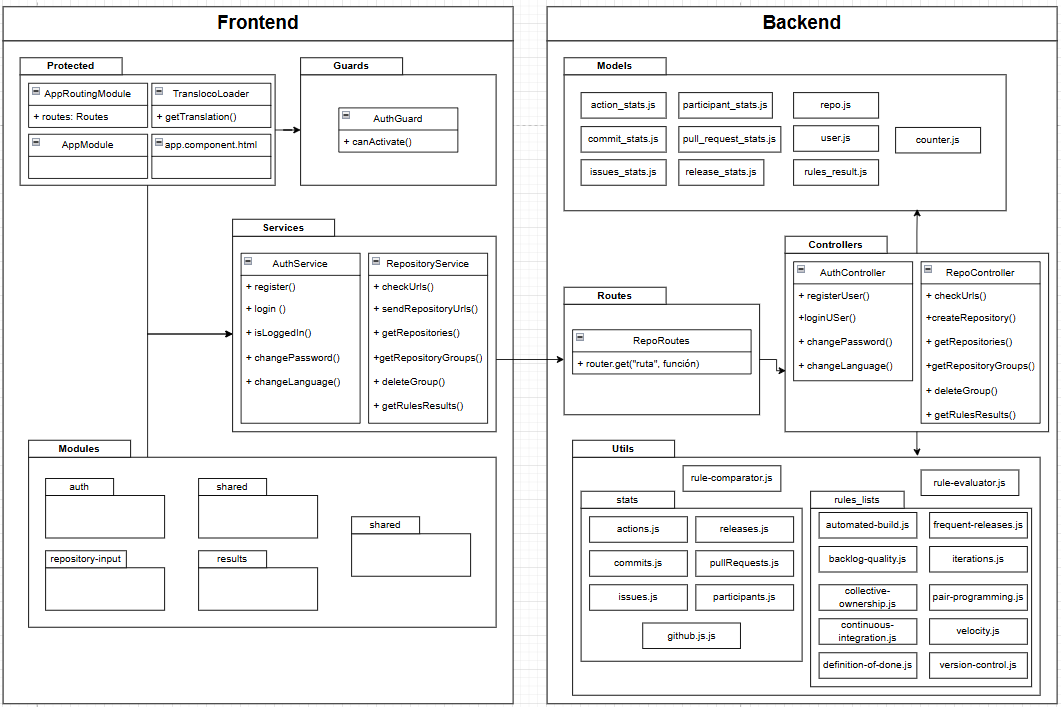
\includegraphics[width=0.8\textwidth]{img/Diagrama-paquetes.png}
\caption{Diagrama del diseño arquitectónico}
\label{fig:DiagramaDirectorios}
\end{figure}

A continuación se detallará en mayor medida las funcionalidades de cada parte tanto del backend como el frontend

\begin{itemize}
    \item \textbf{Frontend}:
    \begin{itemize}
    	\item \textbf{Guards}: Incluye el fichero auth-guard.guard.ts, que se encarga de reforzar la seguridad de acceso a la aplicación bloqueando accesos a las distintas URLs sin haber iniciado sesión
    	\item \textbf{Modules}: Contiene casi toda la lógica del fontend, incluyendo todos los componentes .ts, .html y .css de cada parte de la página web, encargándose estos de definir la lógica, estructura de la página y estilos de maquetación de la misma, respectivamente. Se puede apreciar una mejor representación de su estructura en la figura siguiente. Se compone de las siguientes carpetas:
            \begin{itemize}
                \item \textbf{auth}: Da forma a la pantalla de inicio y usa sus componentes hijos para cambiar entre formulario de registro, inicio de sesión o cambio de contraseña.
                \item \textbf{repository-input}: Se encarga de la pantalla donde el usuario introduce los repositorios y configura el análisis.
                \item \textbf{results}: Muestra la pantalla de los resultados de las prácticas ágiles.
                \item \textbf{statistics}: Muestra la pantalla de comparación de métricas de proceso, que se compone de 2 listas comparativas entre repositorios.
                \item \textbf{shared}: Contiene componentes que usan varias pantallas, como lo son el \textit{header} y el \textit{footer}.
            \end{itemize}
    	\item \textbf{Protected}: Incluye los módulos y componentes más importantes del código, como las definiciones de las rutas, las librerías y componentes a usar, el fichero html principal y el cargador de la librería de traducciones "Transloco".
    	\item \textbf{Services}: Incluye los ficheros auth.service.ts y repository.service.ts, que utilizarán peticiones HttpClient para llamar a las funciones correspondientes de los controladores del backend y utilizar sus funciones.
    \end{itemize}

    \begin{figure}[H]
    \centering
    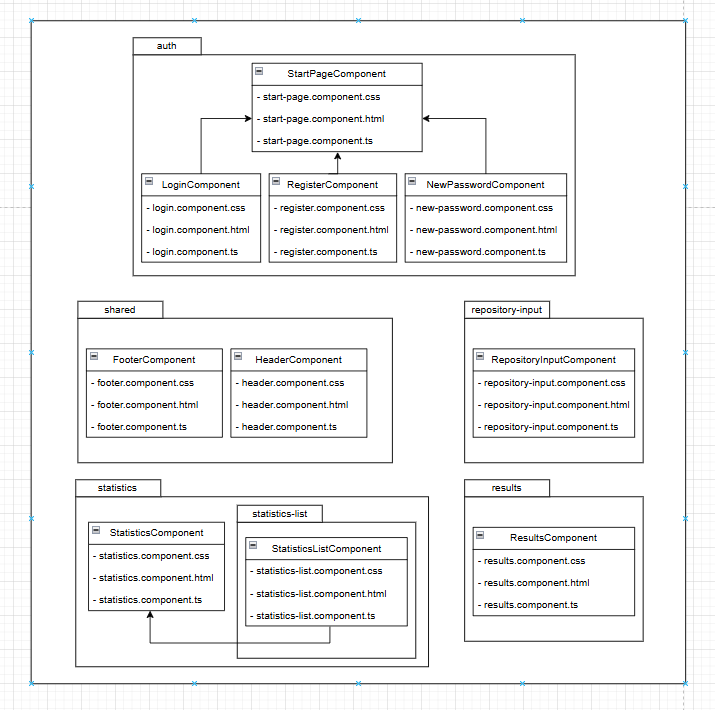
\includegraphics[width=0.8\textwidth]{img/Diagrama-detalle-modules.png}
    \caption{Diagrama del directorio \textbf{modules} del frontend}
    \label{fig:DiagramaDetalleModules}
    \end{figure}
    
    \item \textbf{Backend}:
    \begin{itemize}
    	\item \textbf{controllers}: Se compone de authController.js y repoController.js, que son los ficheros con las funciones principales que definen la lógica general del código relacionado con la autentificación de usuarios y el manejo de repositorios, respectivamente. Para ello utilizarán los modelos definidos en "Models" y las funciones menores definidad en "utils"
        \item \textbf{routes}: Su fichero repoRoutes.js define las rutas que usarán los servicios del frontend para acceder a las funciones de los controllers.
    	\item \textbf{models}: Contiene los ficheros que definen cada tabla de la base de datos a través de la librería mongoose.
    	\item \textbf{utils}: Contiene las funciones secundarias necesarias que usará repoController.js. Hay un fichero y función pequeña para cada tabla de métricas (\textit{commits}, \textit{issues}, etc), junto a un fichero github.js que obtiene datos del repositorio importantes como el título y autor; y para cada práctica ágil definida (Version control, Iterations, etc), además de algunas funciones de ayuda comorule-comparator.js, que compara las medidas de calidad de proceso entre el repositorio principal y los repositorios de referencia para evaluar las reglas
    \end{itemize}
\end{itemize}

La particularidad de haber dividido el código entre frontend y backend refuerza enormemente la flexibilidad y la escalabilidad del diseño, así como la legibilidad y mantenimiento del código.

\subsection{Patrones de diseño}

No toda la flexibilidad, escalabilidad y robustez se deben sólo a la estructura interna del código, sino también a los patrones de diseño \cite{gamma1994design} aplicados. Estos patrones mejoran de la calidad del código y la reutilización de componentes, y refuerzan la legibilidad y mantenibilidad, así como una comunicación más clara entre desarrolladores o, en el caso del desarrollo de este proyecto, la comunicación entre el alumno autor y el tutor del TFG. 

Para el diseño de este proyecto se han tenido en cuenta los principios SOLID \cite{solid_principles} que, junto a ciertos patrones de diseño concretos, han sido de especial utilidad en una arquitectura como lo es la ya descrita de este proyecto. A continuación se detallan los patrones y principios de diseño más relevantes considerados:

\begin{itemize}
    \item \textbf{Patrón fachada}: Este patrón se aplica especialmente en la comunicación entre el frontend y el backend a través de los servicios (AuthService, RepositoryService). Estos actúan como una "fachada" que simplifica el acceso a múltiples funciones complejas del backend.
    \begin{itemize}
        \item \textbf Facilita la interacción del frontend con el backend al ocultar la complejidad de las peticiones HTTP y lógica interna.
        \item \textbf Mejora la cohesión y disminuye el acoplamiento entre componentes.
        \item \textbf Permite modificar el backend sin afectar al frontend, siempre que la fachada (servicio) mantenga su interfaz.
        \item \textbf Aumenta la reutilización y testeo de código, al centralizar la lógica de acceso a datos.
    \end{itemize}
    
    \item \textbf{Principio Abierto / Cerrado}: Este principio se observa en los controladores y módulos, los cuales están diseñados para permitir extensiones (nuevas rutas, pantallas, reglas) sin necesidad de modificar el código ya existente.
    \begin{itemize}
        \item \textbf{Beneficio}: Facilita la adición de nuevas funcionalidades de forma segura.
        \item \textbf{Beneficio}: Reduce el riesgo de introducir errores al mantener el código existente intacto.
        \item \textbf{Beneficio}: Mejora la mantenibilidad y escalabilidad del sistema.
        \item \textbf{Beneficio}: Favorece el desarrollo ágil, permitiendo iteraciones rápidas.
    \end{itemize}
    
    \item \textbf{Patrón Inyección de Dependencias}:  Angular, por diseño, utiliza inyección de dependencias para los servicios (AuthService, RepositoryService, HttpClient, etc.), permitiendo declarar dependencias en los constructores.
    \begin{itemize}
        \item \textbf{Beneficio}: Aumenta la modularidad del código y promueve el bajo acoplamiento.
        \item \textbf{Beneficio}: Mejora la reutilización y mantenimiento del código.
        \item \textbf{Beneficio}: Permite una mayor flexibilidad en la configuración de servicios.
    \end{itemize}
    
    \item \textbf{Principio de Separación de responsabilidades}: Toda la arquitectura se basa en una clara división de responsabilidades: frontend vs backend, componentes vs servicios, controladores vs modelos, etc.
    \begin{itemize}
        \item \textbf{Beneficio}: Mejora la legibilidad del código al estar organizado por función.
        \item \textbf{Beneficio}: Permite a varios desarrolladores trabajar en paralelo en diferentes áreas del sistema.
        \item \textbf{Beneficio}: Reduce errores al evitar dependencias innecesarias entre módulos.
        \item \textbf{Beneficio}: Favorece la reutilización de módulos y componentes en otros proyectos.
    \end{itemize}
    
    \item \textbf{Patrón Controlador}: Utilizado en el backend para organizar la lógica relacionada con diferentes dominios (AuthController, RepoController). Cada controlador es responsable de orquestar las funciones relacionadas con una entidad del sistema.
    \begin{itemize}
        \item \textbf{Beneficio}: Centraliza la lógica de cada parte del sistema, facilitando su entendimiento y modificación.
        \item \textbf{Beneficio}: Permite escalar el sistema con facilidad al añadir nuevos controladores según se necesiten.
        \item \textbf{Beneficio}: Mejora la trazabilidad de errores
        \item \textbf{Beneficio}: Favorece el desacoplamiento entre la lógica de negocio y la lógica de acceso a datos.
    \end{itemize}
    
    \item \textbf{Patrón decorador}: En Angular se emplea el patrón decorador mediante anotaciones como @Component, @Injectable, @Input, @Output, que permiten añadir información a las clases, propiedades o métodos sin modificar directamente su implementación.
    \begin{itemize}
        \item \textbf{Beneficio}: Permite extender funcionalidades de manera flexible sin modificar el código original.
        \item \textbf{Beneficio}: Aumenta la legibilidad y organización del código, permitiendo declarar claramente el propósito de cada clase o propiedad.
        \item \textbf{Beneficio}: Mejora la reutilización de componentes a través de la configuración por propiedades decoradas (@Input(), usado en \textbf{StatisticsListComponent}).
    \end{itemize}
\end{itemize}

\section{Diseño procedimental}
En esta sección se describirá el flujo a seguir en las tareas más relevantes que se hacen en la aplicación mediante los \textbf{Casos de Uso (CU)} definidos previamente

\subsection*{CU1 - Creación y acceso a la cuenta}

Este caso de uso permite al usuario crear una cuenta en la aplicación o acceder mediante inicio de sesión. Está dirigido a nuevos usuarios o a aquellos que desean autenticarse. El sistema valida la información antes de registrar o permitir el acceso como se puede ver en la figura~\ref{fig:DiagramaCU1})

\textbf{Pasos que sigue el CU:}
\begin{enumerate}
  \item El usuario accede a la página de registro o inicio de sesión.
  \item Introduce su usuario y contraseña.
  \item El sistema verifica los datos ingresados.
  \item Según el caso, se crea una nueva cuenta o se otorga acceso.
\end{enumerate}

\begin{figure}[H]
\centering
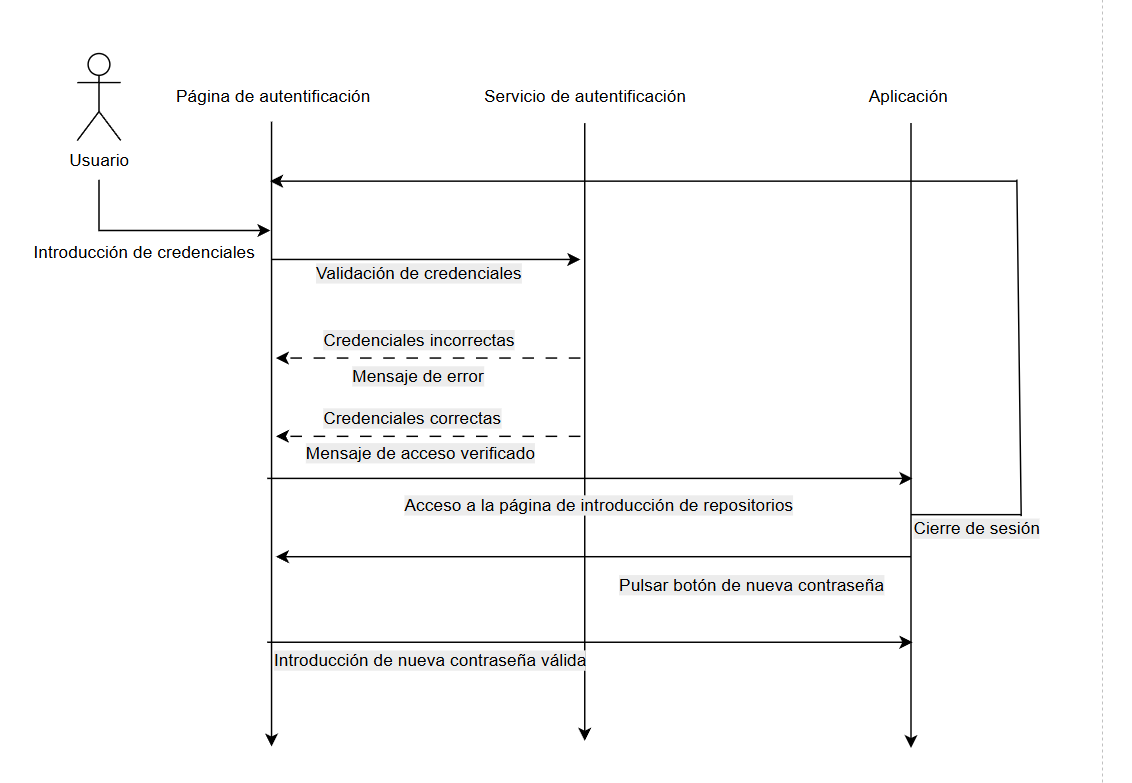
\includegraphics[width=0.8\textwidth]{img/DiagramaCU1.png}
\caption{Diagrama del caso de uso CU1}
\label{fig:DiagramaCU1}
\end{figure}

\subsection*{CU2 - Configuración de la cuenta}

Permite al usuario modificar su configuración de cuenta, como el idioma o la contraseña. Es necesario haber iniciado sesión previamente. El sistema valida y aplica los cambios, tal como se muestra en la figura~\ref{fig:DiagramaCU2}.

\textbf{Pasos que sigue el CU:}
\begin{enumerate}
  \item El usuario accede a la sección de configuración.
  \item Selecciona si desea cambiar la contraseña o el idioma.
  \item El sistema valida los datos ingresados y aplica los cambios.
\end{enumerate}

\begin{figure}[H]
\centering
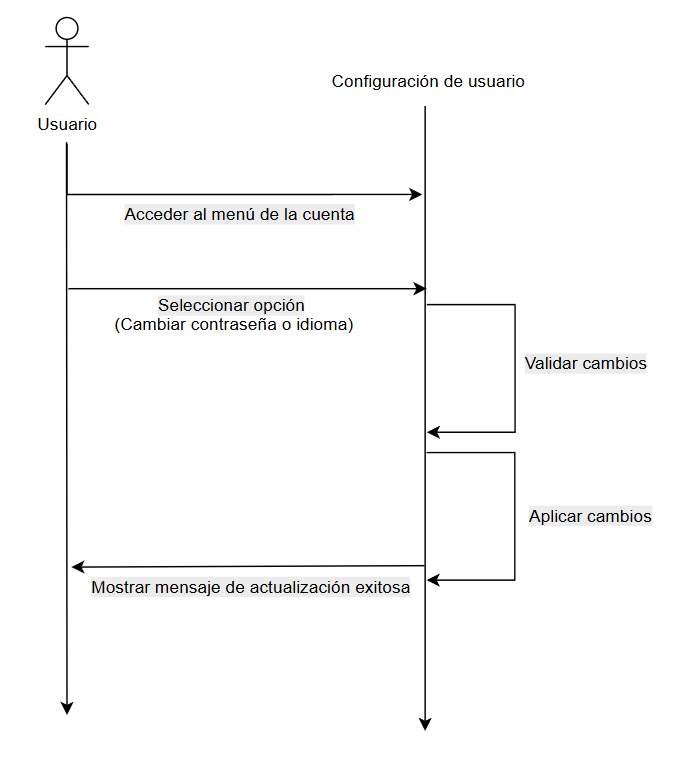
\includegraphics[width=0.8\textwidth]{img/DiagramaCU2.png}
\caption{Diagrama del caso de uso CU2}
\label{fig:DiagramaCU2}
\end{figure}

\subsection*{CU3 - Introducción y validación de URLs de repositorios}

Este caso de uso permite al usuario introducir una o más URLs de repositorios GitHub para su posterior análisis. El sistema se encarga de validar tanto la estructura como el acceso. La figura~\ref{fig:DiagramaCU3-CU6-CU7} describe un flujo de introducción y validación de URLs de repositorios para su posterior visualización.

\textbf{Pasos que sigue el CU:}
\begin{enumerate}
  \item El usuario introduce una o varias URLs.
  \item El sistema valida su formato y accesibilidad.
  \item Si las URLs no son correctamente validadas saltará un mensaje de error. En caso contrario, el análisis se iniciará cuando el usuario pulse el botón..
\end{enumerate}

\subsection*{CU4 - Configuración del análisis de repositorios}

Este caso de uso permite definir cómo se analizarán los datos de los repositorios previamente introducidos. El usuario puede personalizar fechas, tipos de intervalos y métricas. Cada paso incluye validaciones, y al final se habilita la opción de comparar (ver figura~\ref{fig:DiagramaCU4}).

\textbf{Pasos que sigue el CU:}
\begin{enumerate}
  \item El usuario elige el número de días sobre el cual se basarán las medidas de calidad que reflejan medias estadísticas.
  \item El usuario elige entre analizar los repositorios al completo o por intervalos de tiempo.
  \item El usuario elige en qué intervalos de tiempo realizar el análisis.
  \item Se validan las entradas y se habilita el botón \textit{Comparar}.
\end{enumerate}

\begin{figure}[H]
\centering
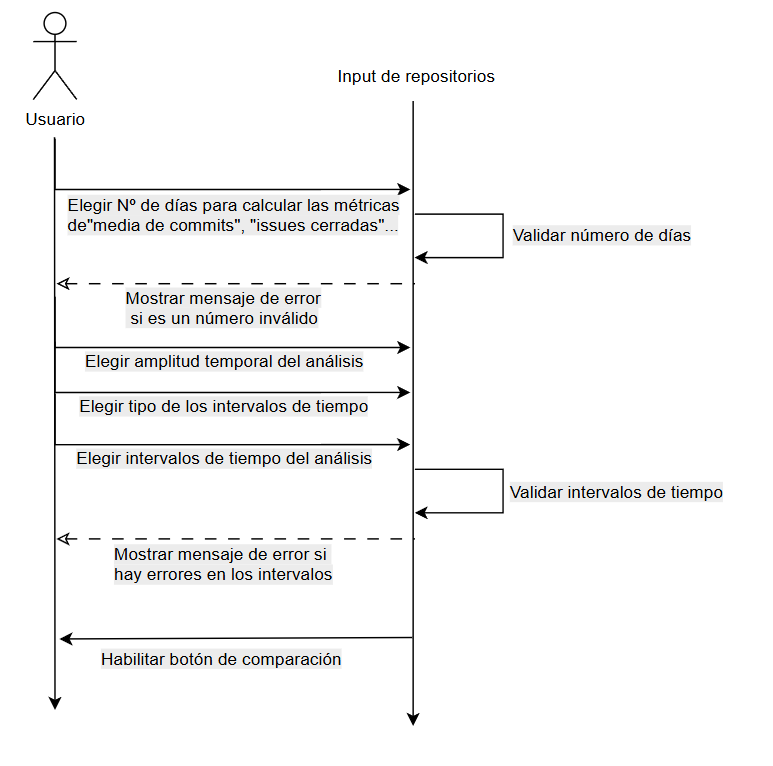
\includegraphics[width=0.8\textwidth]{img/DiagramaCU4.png}
\caption{Diagrama del caso de uso CU4}
\label{fig:DiagramaCU4}
\end{figure}

\subsection*{CU5 - Gestión de grupos de repositorios de referencia}

Este caso de uso permite gestionar grupos de repositorios previamente guardados como referencia comparativa. El usuario puede cargarlos o eliminarlos, siempre y cuando tenga al menos un grupo guardado. (Ver figura~\ref{fig:DiagramaCU5})

\textbf{Pasos que sigue el CU:}
\begin{enumerate}
  \item El usuario accede a la gestión de grupos de repositorios.
  \item Selecciona uno para cargarlo.
  \item Opcionalmente elimina uno o más grupos.
\end{enumerate}

\begin{figure}[H]
\centering
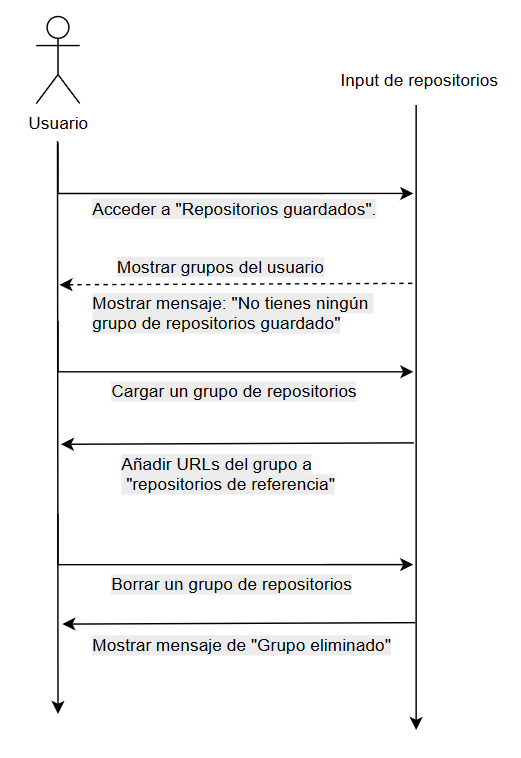
\includegraphics[width=0.8\textwidth]{img/DiagramaCU5.png}
\caption{Diagrama del caso de uso CU5}
\label{fig:DiagramaCU5}
\end{figure}

\subsection*{CU6 - Visualización de prácticas ágiles}

Permite al usuario visualizar los resultados de un análisis automático de prácticas ágiles basado en las medidas de calidad de proceso extraídas de los repositorios. Se presentan los resultados en forma gráfica y textual, indicando qué prácticas se cumplen, en qué medida, y en qué aspectos hay lugar para mejoras. Esto puede observarse en la figura~\ref{fig:DiagramaCU3-CU6-CU7}, junto a la posibilidad de que el usuario cambie de pantalla y vuelva a la de este caso de uso o pase a la del CU7.

\textbf{Pasos que sigue el CU:}
\begin{enumerate}
  \item El sistema muestra los resultados del uso de prácticas ágiles del análisis en forma gráfica y textual.
  \item El usuario revisa qué prácticas de agilidad se cumplen, cuáles no, y los motivos.
\end{enumerate}

\subsection*{CU7 - Comparación de medidas de calidad de proceso}

Este caso de uso permite al usuario comparar visualmente las métricas de calidad de su repositorio analizado con aquellas de uno o más repositorios de referencia previamente cargados. El sistema genera listas comparativas para facilitar la interpretación. Esta funcionalidad, junto a las de los casos de uso CU3 y CU6 se detalla gráficamente en la figura~\ref{fig:DiagramaCU7} siguiendo un flujo detallado del proceso de validación de URLs de repositorios para después ver los resultados.

\textbf{Pasos que sigue el CU:}
\begin{enumerate}
  \item El usuario accede a la sección de comparación.
  \item El sistema genera y muestra listas comparativas con las métricas seleccionadas del repositorio actual y los de referencia.
  \item El usuario analiza los resultados para evaluar el estado de su proyecto.
\end{enumerate}

\begin{figure}[H]
\centering
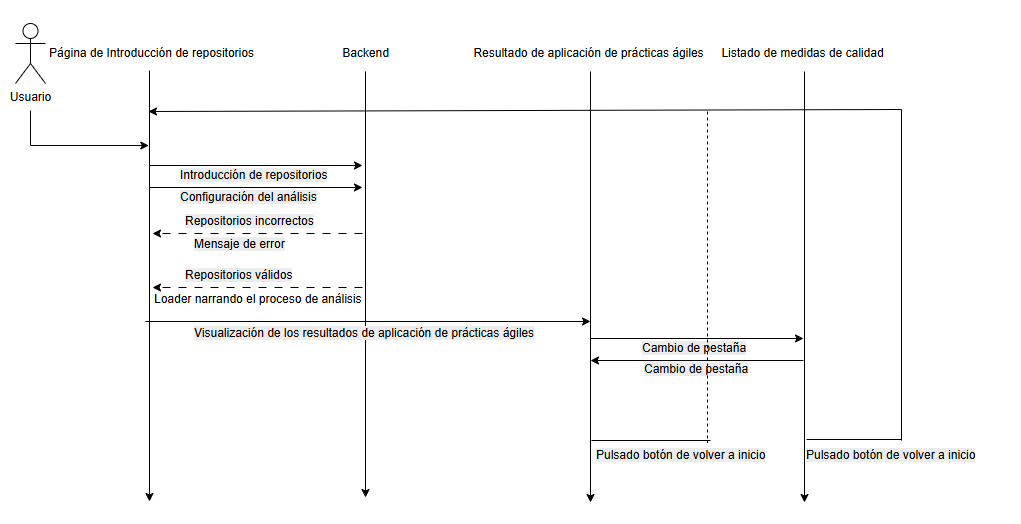
\includegraphics[width=0.8\textwidth]{img/DiagramaCU3-CU6-CU7.png}
\caption{Diagrama del caso de uso CU7}
\label{fig:DiagramaCU3-CU6-CU7}
\end{figure}